\section{Erstellung des Sechobjects}

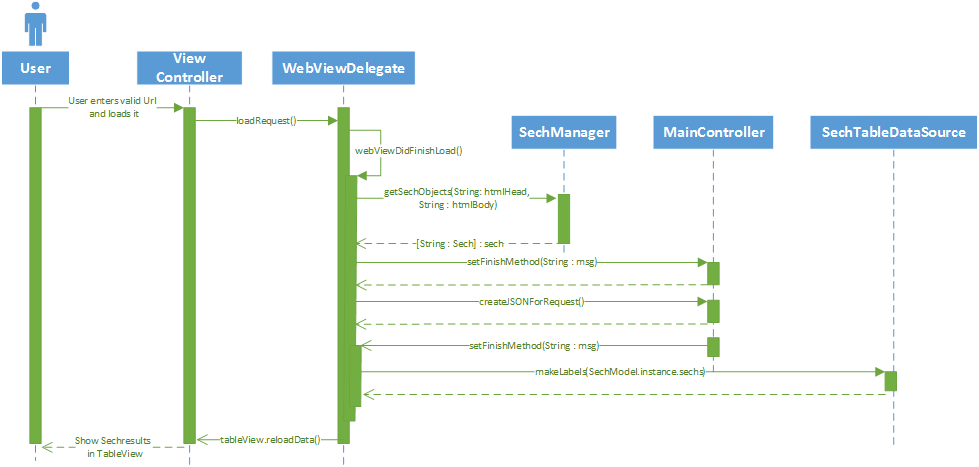
\includegraphics[scale=0.6]{sechobject.png}

\textbf{Ablauf:}
Sobald der User eine g�ltige URL eingibt und l�dt, wird die Laderoutine \Verb|loadRequest()|
angesto�en. Ist die Seite fertig geladen wird in der Delegatemethode \Verb|webViewDidFinishLoad()|
des WebViewDelegates das Auslesen bzw. Laden der \SEACH-Tags begonnen.
Dem \SEACH-Manager wird der HTML-Head und Body der eben geladenen Website �bergeben und es
werden mit Hilfe des HTMLManagers \SEACH-Objekte erstellt. Diese \SEACH-Objekte werden in einem
Dictionary zur�ckgegeben.
Die \Verb|setFinishMethod()|-Methode bereitet den MainController darauf vor, asynchron eine Methode
im WebViewDelegate aufzurufen, sobald die \SEACH-Objekte durch die Response erweitert worden
sind. Der Prozess der EEXCESS-Abfrage wird dann durch die Methode \Verb|createJSONForRequest()| mit
dem Parameter des \SEACH-Dictionarys angesto�en. Sobald dann die Elemente erweitert wurden ruft
der MainController die \Verb|setFinishMethod()| des WebViewDelegates auf und die Liste der \SEACH-Tags
im UI wird aktualisiert.
